\documentclass[12pt]{article}
\usepackage[margin = 1.5in]{geometry}
\setlength{\parindent}{0in}
\usepackage{amsfonts, amssymb, amsthm, mathtools, tikz, qtree, float}
\usepackage{algpseudocode, algorithm, algorithmicx}
\usepackage{ae, aecompl, color}
\usepackage{wrapfig}
\usepackage{multicol, multicol, array}
\usepackage{imakeidx}
\makeindex[columns=2, title=Indices, intoc]

\usepackage[pdftex, pdfauthor={Charles Shen}, pdftitle={CS 350: Operating Systems}, pdfsubject={Lecture notes from CS 350: at the University of Waterloo}, pdfkeywords={course notes, notes, Waterloo, University of Waterloo}, pdfproducer={LaTeX}, pdfcreator={pdflatex}]{hyperref}
\usepackage{cleveref}

\DeclarePairedDelimiter{\set}{\lbrace}{\rbrace}
\definecolor{darkish-blue}{RGB}{25,103,185}

\hypersetup{
  colorlinks,
  citecolor=darkish-blue,
  filecolor=darkish-blue,
  linkcolor=darkish-blue,
  urlcolor=darkish-blue
}

\theoremstyle{plain}
\newtheorem{theorem}{Theorem}[subsection]

\theoremstyle{definition}
\newtheorem{proposition}[theorem]{Proposition}
\newtheorem{corollary}[theorem]{Corollary}
\newtheorem{lemma}[theorem]{Lemma}
\newtheorem{ex}[theorem]{Example}
\newtheorem*{ex*}{Example}
\newtheorem{defn}{Definition}

\crefname{ex}{Example}{Example}

\setlength{\marginparwidth}{1.5in}
\newcommand{\lecture}[1]{
  \marginpar{{
    \footnotesize $\leftarrow$ \underline{#1}}
  }
}

\newcommand{\defnterm}[1]{\textbf{\textcolor{teal}{#1}}\index{#1}}

\newcolumntype{L}[1]{>{\raggedright\let\newline\\\arraybackslash\hspace{0pt}}m{#1}}
\newcolumntype{C}[1]{>{\centering\let\newline\\\arraybackslash\hspace{0pt}}m{#1}}
\newcolumntype{R}[1]{>{\raggedleft\let\newline\\\arraybackslash\hspace{0pt}}m{#1}}

\allowdisplaybreaks

\makeatletter
\def\blfootnote{\gdef\@thefnmark{}\@footnotetext}
\makeatother

%%%%%%%%%%%%%%%%%%%%%
%% D O C U M E N T %%
%%%%%%%%%%%%%%%%%%%%%

\begin{document}
\let\ref\Cref
\pagenumbering{roman}

\title{\bf{CS 350: Operating Systems}}
\date{Fall 2016, University of Waterloo \\ \center Notes written from Gregor Richards's lectures.}
\author{Charles Shen}

\blfootnote{Feel free to email feedback to me at
\href{mailto:ccshen902@gmail.com}{ccshen902@gmail.com}.}

\maketitle
\thispagestyle{empty}
\newpage
\tableofcontents
\newpage
\pagenumbering{arabic}

%%%%%%%%%%%%%%%%%%
%% INTRODUCTION %%
%%%%%%%%%%%%%%%%%%
\section{Introduction}
There are three views of an operating system:
\begin{enumerate}
  \item[1.] \defnterm{Application View} (\ref{app_view_OS}): what service does it provide?
  \item[2.] \defnterm{System View} (\ref{sys_view_OS}): what problems does it solve?
  \item[3.] \defnterm{Implementation View} (\ref{impl_view_OS}): how is it built?
\end{enumerate}
\emph{An operating system is part cop, part facilitator}. \\

\defnterm{kernel}: The operating system kernel is the part of the operating system that responds to system calls, interrupts and exception. \\

\defnterm{operating system} (OS): The operating system as a whole includes the kernel, and may include other related programs that provide services for application such as utility programs, command interpreters, and programming libraries.

\subsection{Application View of an Operating System}\label{app_view_OS}
The OS provides an execution environment for running programs.
\begin{itemize}
  \item The execution environment provides a program with the processor time and memory space that it needs to run.
  \item The execution environment provides interfaces through which a program can use networks, storage, I/O devices, and other system hardware components. \\
  Interfaces provide a simplified, abstract view of hardware to application programs.
  \item The execution environment isolates running programs from one another and prevents undesirable interactions among them.
\end{itemize}

\subsection{System View of an Operating System}\label{sys_view_OS}
The OS manages the hardware resources of a computer system.
\begin{itemize}
  \item Resources include processors, memory, disks and other storage devices, network interfaces, I/O devices such as keyboards, mice and monitors, and so on.
  \item The operating system allocates resources among running programs. \\
  It controls the sharing of resources among programs.
  \item The OS itself also uses resources, which it must share with application programs.
\end{itemize}

\subsection{Implementation View of an Operating System}\label{impl_view_OS}
The OS is a concurrent, real-time program.
\begin{itemize}
  \item Concurrency arises naturally in an OS when it supports concurrent applications, and because it must interact directly with the hardware.
  \item Hardware interactions also impose timing constraints.
\end{itemize}

\subsection{Operating System Abstractions}
The execution environment provided by the OS includes a variety of abstract entities that can be manipulated by a running program. \\
Examples:
\begin{itemize}
  \item \textbf{files and file systems}: abstract view of secondary storage
  \item \textbf{address spaces}: abstract view of primary memory
  \item \textbf{processes, threads}: abstract view of program execution
  \item \textbf{sockets, pipes}: abstract view of network or other message channels
\end{itemize}

%%%%%%%%%%%%%%%%%%%%%%%%%%%%%
%% THREADS AND CONCURRENCY %%
%%%%%%%%%%%%%%%%%%%%%%%%%%%%%
\newpage
\section{Threads and Concurrency}
Threads provide a way for programmers to express \emph{concurrency} in a program. \\
A normal \emph{sequential program} consists of a single thread of execution. \\
In threaded concurrent programs, there are multiple threads of executions that are all occurring at the same time.

\subsection{OS/161's Thread Interface}
Create a new thread:
\begin{verbatim}
int thread_fork(
  const char *name,             // name of new thread
  struct proc *proc,            // thread's process
  void (*func)                  // new thread's function
    (void *, unsigned long),
  void *datat1,                 // function's first param
  unsigned long data2           // function's second param
);
\end{verbatim}

Terminating the calling thread: \\
\begin{verbatim}
void thread_exit(void);
\end{verbatim}

Voluntarily yield execution: \\
\begin{verbatim}
void thread_yield(void);
\end{verbatim}


\newpage
\section{Processes and System Calls}

\newpage
\section{Assignment 2A Review}

\newpage
\section{Virtual Memory}
\subsection{Physical Memory and Addresses}
\begin{figure}[!h]
  \centering
  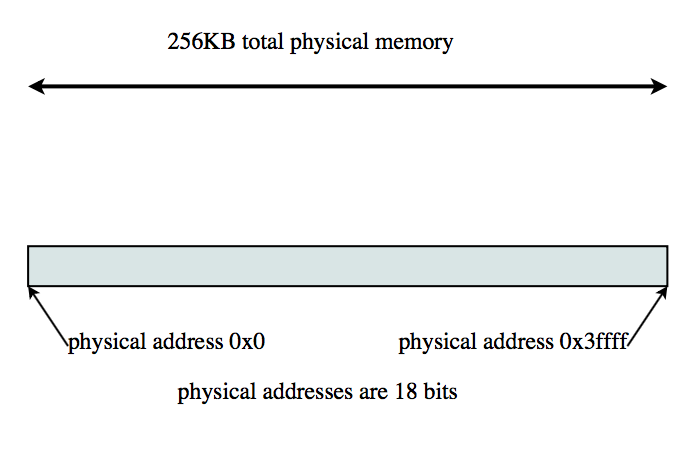
\includegraphics[scale=0.65]{pictures/phys_mem.png}
  \caption{An example physical memory, $P = 18$}
  \label{fig:phys_mem}
\end{figure}
If physical addresses have $P$ \emph{bits}, the maximum amount of addressable physical memory is $2^{P}$ \emph{bytes} (assuming a byte-addressable machine).
\begin{itemize}
  \item Sys/161 MIPS processor uses 32 bit physical addresses ($P = 32$) $\Rightarrow$ maximum physical memory size of $2^32$ bytes, or 4GB
  \item Larger values of $P$ are common on modern processors, e.g., $P = 48$, which allows 256TB of physical memory to be addressed
\end{itemize}

The actual amount of physical memory on a machine may be less than the maximum amount that can be addressed.

\subsection{Virtual Memory and Addresses}
\begin{figure}[!h]
  \centering
  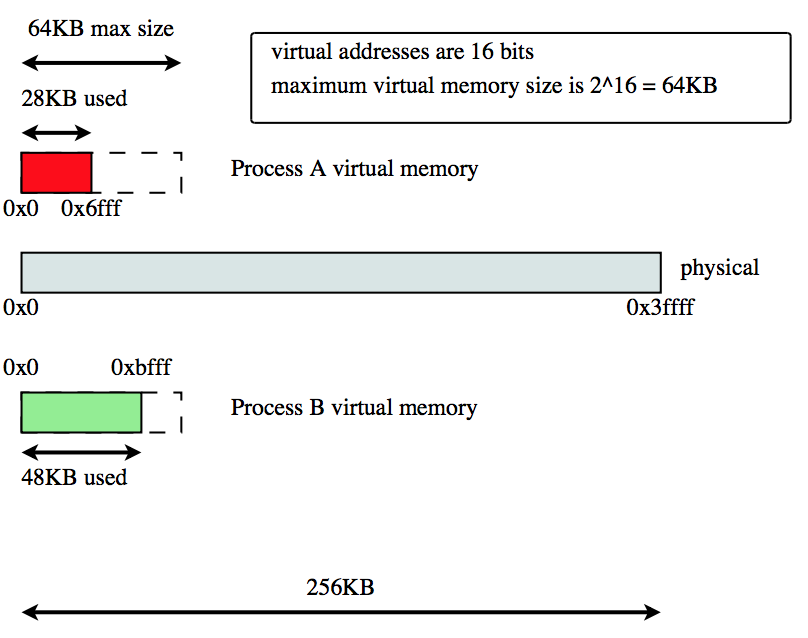
\includegraphics[scale=0.65]{pictures/v_mem.png}
  \caption{An example of virtual memory, $V = 16$}
  \label{fig:v_mem}
\end{figure}
The kernel provides a separate, private \emph{virtual} memory for each process. \\
The virtual memory of a process holds the code, data, and stack for the program that is running in that process. \\
If virtual addresses are $V$ bits, the \emph{maximum} size of a virtual memory is $2^{V}$ bytes.
\begin{itemize}
  \item For the MIPS, $V = 32$
\end{itemize}
Running applications see only virtual addresses, e.g.,
\begin{itemize}
  \item program counter and stack pointer hold \emph{virtual addresses} of the next instruction and the stack
  \item pointers to variables are \emph{virtual addresses}
  \item jumps/branches refer to \emph{virtual addresses}
\end{itemize}
Each process is isolated in its virtual memory, and cannot access other process' virtual memories.

\subsection{Address Translation}
Each virtual memory is mapped to a different part of physical memory. \\
Since virtual memory is not real, when an process tries to access (load or store) a virtual address, the virtual address is \emph{translated} (mapped) to its corresponding physical address, and the load or store is performed in physical memory. \\
Address translation is performed in hardware, using information provided by the kernel.

\subsection{Address Translation for Dynamic Relocation}
\begin{figure}[!h]
  \centering
  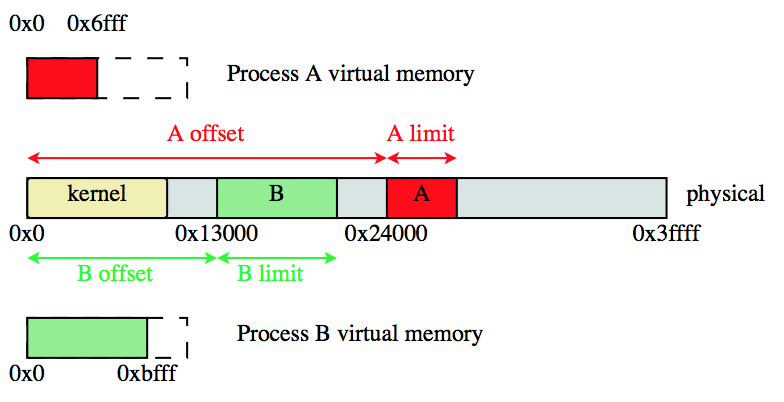
\includegraphics[scale=0.6]{pictures/dyn_reloc.png}
  \caption{Example of dynamic relocation}
  \label{fig:figure1}
\end{figure}
CPU includes a \emph{memory management unit} (MMU), with a \emph{relocation register} and a \emph{limit register}.
\begin{itemize}
  \item relocation register holds the physical offset ($R$) for the running process' virtual memory
  \item limit register holds the size $L$ of the running process' virtual memory
\end{itemize}
To translate a virtual address $v$ to a physical address $p$:
\begin{align*}
&\texttt{if } v \geq L \texttt{ then generate exception} \\
&\texttt{else} \\
&\qquad p \leftarrow v + R
\end{align*}
Translation is done in hardware by the MMU. \\
The kernel maintains a separate $R$ and $L$ for each process, and changes the values in the MMU registers when there is a context switch between processes. \\

\begin{ex*}
$v = \texttt{0x102c} \qquad p = \texttt{0x102c} + \texttt{0x24000} = \texttt{0x2502c}$ \\
$v = \texttt{0x8800} \qquad p = \texttt{exception}$ since $\texttt{0x8800} \geq \texttt{0x7000}$
\end{ex*}

\subsection{Properties of Dynamic Relocation}
Each virtual address space corresponds to a \emph{contiguous range of physical addresses}. \\
The kernel is responsible for deciding \emph{where} each virtual address space should map in physical memory.
\begin{itemize}
  \item the OS must track which part of physical memory are in use, and which parts are free
  \item since different address spaces may have different sizes, the OS must allocate/deallocate variable-sized chunks of physical memory
  \item hence creates potential for \emph{fragmentation} of physical memory
\end{itemize}

\subsection{Paging: Physical Memory}
Physical memory is divided into fixed-size chunks called \emph{frames} or \emph{physical pages}.
\begin{figure}[!h]
  \centering
  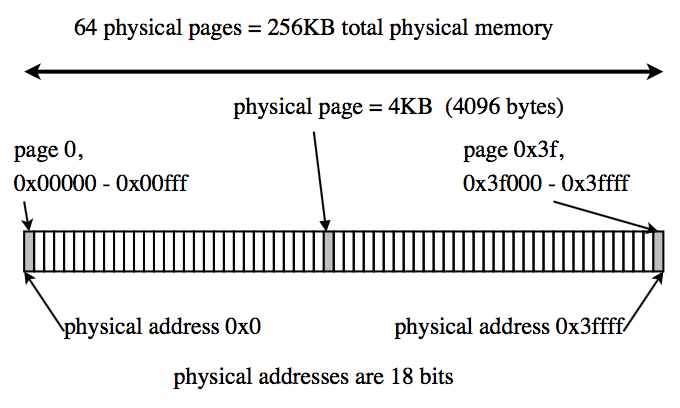
\includegraphics[scale=0.7]{pictures/paging_phys_mem.png}
  \caption{The frame size if $2^{12}$ bytes (4KB)}
  \label{fig:p_phys_mem}
\end{figure}

\subsection{Paging: Virtual Memory}
Virtual memories are divided into fixed-size chunks called \emph{pages}. \\
Page size is equal to frame size.
\begin{figure}[!h]
  \centering
  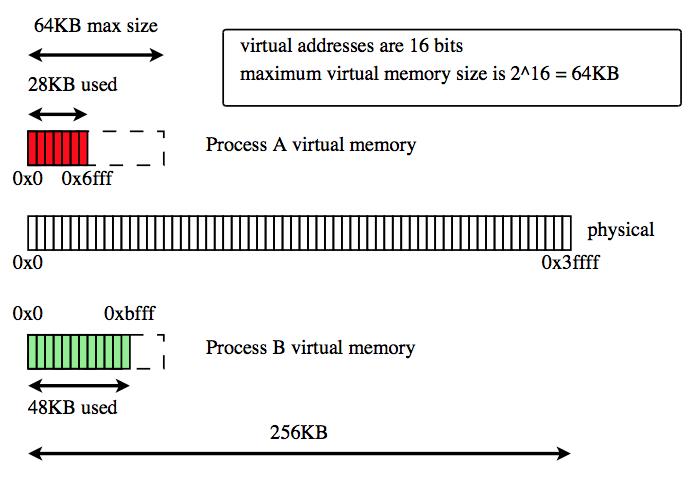
\includegraphics[scale=0.8]{pictures/paging_v_mem.png}
  \caption{Page size is 4KB here}
  \label{fig:p_v_mem}
\end{figure}

\subsection{Paging: Address Translation}
\begin{figure}[!h]
  \centering
  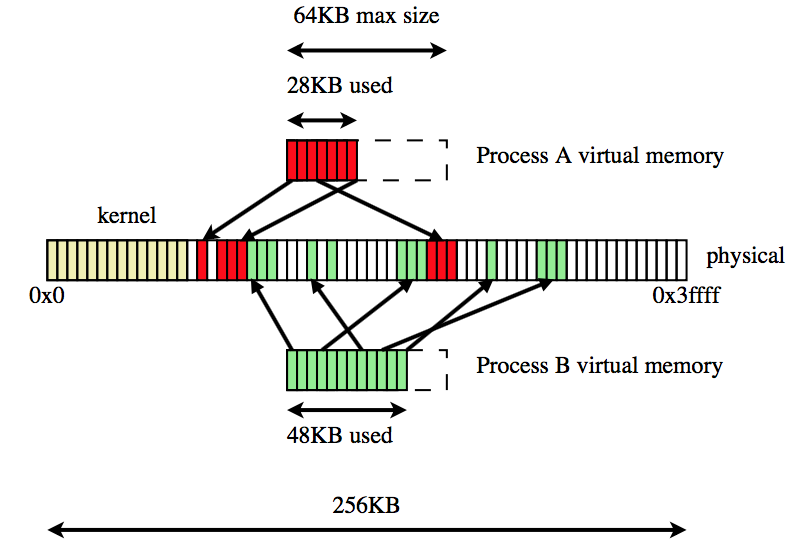
\includegraphics[scale=0.7]{pictures/p_translation.png}
  \label{fig:figure1}
\end{figure}
Each page maps to a different frame.
Any page can map to any frame.

\subsection{Paging: Address Translation}
The MMU includes a \emph{page table base register} which points to the page table for the current process. \\

How the MMU translate a virtual address:
\begin{enumerate}
  \item[1.] determines the \emph{page number} and \emph{offset} of the virtual address
  \begin{itemize}
    \item page number is the virtual address divided by the page size
    \item offset is the virtual address modulo the page size
  \end{itemize}
  \item[2.] looks up the page's entry (PTE) in the current process page table, using the page number
  \item[3.] if the PTE is not valid, raise an exception
  \item[4.] otherwise, combine page's frame number from the PTE with the offset to determine the physical address \\
\end{enumerate}

\newpage
\section{Scheduling}

\newpage
\section{Devices and Device Management}

\newpage
\section{File Systems}

\newpage
\section{Interprocess Communications and Networking}

\clearpage
\printindex
\end{document}

%%%%%%%%%%%%%%%%%%%%%
%% D O C U M E N T %%
%%%%%%%%%%%%%%%%%%%%%
